% Generated by jats2tex@0.11.1.0
% template.yaml 2.1.3.3 (comentários da Francine)
\documentclass{article}
\usepackage{scielo}

\newcommand{\journalid}{Rev Saude Publica}
\newcommand{\journaltitle}{Revista de Saúde Pública}
\newcommand{\abbrevjournaltitle}{Rev. Saúde Pública}
\newcommand{\issnppub}{0034-8910}
\newcommand{\issnepub}{1518-8787}
\newcommand{\publishername}{Faculdade de Saúde Pública da Universidade de São
Paulo}
\newcommand\articledoi{DOI 10.1590/S0034-8910.2013047004402}
\def\subject{Prática de Saúde Pública}
\title{Necessidade de implantar programa nacional de segurança do
paciente no Brasil\titlegroup{}}
\newcommand{\transtitlees}{Necesidad de implantar programa nacional de seguridad
del paciente en
Brasil}
\author[I]{Capucho, Helaine Carneiro}
\author[II]{Cassiani, Silvia Helena De Bortoli}
\affil[I]{Departamento de Gestão e Incorporação de Tecnologias em
Saúde, Secretaria de Ciência, Tecnologia e Insumos
Estratégicos, Ministério da Saúde}
\affil[II]{Departamento de Enfermagem Geral e
Especializada, Escola de Enfermagem de Ribeirão Preto, Universidade de São
Paulo}
\def\authornotes{Correspondência | Correspondence : Helaine Carneiro Capucho.
Esplanada dos
Ministérios. Bloco G Edifício Sede 9º andar Sala 949. 70058-900 Brasília, DF,
Brasil.
E-mail: helaine.capucho@saude.gov.br
Os autores declaram não haver conflito de interesses.
}
\date{ 08 2013}
\def\volume{47}
\def\issue{4}
\def\fpage{791}
\def\lpage{798}
\newcommand{\datereceived}{4-6-2012}
\newcommand{\dateaccepted}{21-6-2012}
\newcommand{\cclicense}{\ccbync}
\newcommand{\kwdgroup}{Segurança do Paciente, Avaliação de Programas e Projetos
de Saúde, Sistema Único de Saúde, Garantia da Qualidade dos Cuidados de Saúde}
\newcommand{\kwdgroupes}{Seguridad del Paciente, Evaluación de Programas y
Proyectos de Salud, Sistema Único de Salud, Garantía de la Calidad de Atención
de Salud}\newcommand{\ack}{
The authors wish to thank the School of Nursing at the University of São Paulo
and FAPESP that financed and subsididized this study under process number
2012/02700-7, with dispatch issued on May 9, 2012.
}
%%% Nota fn1 %%%%%%%%%%%%%%%%%%%%%%%%%%%%%%%%%%%%%%%%%%%%%%%%%%%%%%%%
\expandafter\newcommand\csname fn1\endcsname{
World Health Organization. APPS web-based registration mechanism open. Geneva;
2012
[citado 2012 jun 2]. Disponível em: http://www.who.int/patientsafety/en/
}
%%% Nota fn2 %%%%%%%%%%%%%%%%%%%%%%%%%%%%%%%%%%%%%%%%%%%%%%%%%%%%%%%%
\expandafter\newcommand\csname fn2\endcsname{
Capucho HC. Sistemas manuscrito e informatizado de notificação voluntária de
incidentes
em saúde como base para a cultura de segurança do paciente [tese de doutorado].
São Paulo:
Escola de Enfermagem de Ribeirão Preto da USP; 2012.
}
%%% Nota fn3 %%%%%%%%%%%%%%%%%%%%%%%%%%%%%%%%%%%%%%%%%%%%%%%%%%%%%%%%
\expandafter\newcommand\csname fn3\endcsname{
Ministério da Saúde. Portaria GM/MS nº 529, de 1 de abril de 2013. Institui o
Programa
Nacional de Segurança do Paciente (PNSP). \textit{Diario Oficial Uniao}
. 2 abr
2013;Seção1:43-4.
}
%%% Nota fn4 %%%%%%%%%%%%%%%%%%%%%%%%%%%%%%%%%%%%%%%%%%%%%%%%%%%%%%%%
\expandafter\newcommand\csname fn4\endcsname{
Petramale CA. O projeto dos hospitais sentinela e a gerência de risco sanitário
hospitalar. In: Capucho HC, Carvalho FD, Cassiani SHB. Farmacovigilância -
Gerenciamento
de Riscos da Terapia Medicamentosa para a Segurança do Paciente. São Caetano do
Sul:
Editora Yendis. 2001. p. 191-224.
}
%%% Nota fn5 %%%%%%%%%%%%%%%%%%%%%%%%%%%%%%%%%%%%%%%%%%%%%%%%%%%%%%%%
\expandafter\newcommand\csname fn5\endcsname{
Ministério da Saúde. Portaria nº 396, de 4 de março de 2011 Institui o projeto
de
formação e melhoria da qualidade de rede de saúde (Quali-SUS-Rede) e suas
diretrizes
operacionais gerais. \textit{Diario Oficial Uniao}
. 9 mar 2011.
}
%%% Nota fn6 %%%%%%%%%%%%%%%%%%%%%%%%%%%%%%%%%%%%%%%%%%%%%%%%%%%%%%%%
\expandafter\newcommand\csname fn6\endcsname{
Ministério da Saúde. Índice de Desempenho do SUS – IDSUS. Brasília (DF); 2011
[citado
2012 jun 2]. Disponível em:
http://portal.saude.gov.br/portal/saude/area.cfm?id\_{}area=1080
}
%%% Nota fn7 %%%%%%%%%%%%%%%%%%%%%%%%%%%%%%%%%%%%%%%%%%%%%%%%%%%%%%%%
\expandafter\newcommand\csname fn7\endcsname{
Brasil. Lei nº 12.401, de 28 de abril de 2011. Altera a Lei nº 8.080, de 19 de
setembro
de 1990, para dispor sobre a assistência terapêutica e a incorporação de
tecnologia em
saúde no âmbito do Sistema Único de Saúde - SUS. \textit{Diario Oficial Uniao}
.
29 abr 2011:1.
}
%%% Nota fn8 %%%%%%%%%%%%%%%%%%%%%%%%%%%%%%%%%%%%%%%%%%%%%%%%%%%%%%%%
\expandafter\newcommand\csname fn8\endcsname{
World Health Organization. WHO launches ‘Nine patient safety solutions. Geneva;
2007
[citado 2012 jun 2]. Disponível em:
http://www.who.int/mediacentre/news/releases/2007/pr22/en/index.html
}
%%% Nota %%%%%%%%%%%%%%%%%%%%%%%%%%%%%%%%%%%%%%%%%%%%%%%%%%%%%%%%
\expandafter\newcommand\csname \endcsname{
Trabalho baseado na tese de doutorado, de Capucho H. C., intitulada: “Sistemas
manuscrito
e informatizado de notificação voluntária de incidentes em saúde como base para
a cultura
de segurança do paciente”, apresentada à Escola de Enfermagem de Ribeirão Preto
da
Universidade de São Paulo, em 2012.
}

\begin{document}
\selectlanguage{portuges}
\newcommand{\lingua}{Português}
\maketitle
\tableofcontents

\begingroup
\renewcommand{\section}[1]{\subsection*{#1}}

\begin{abstract}

O objetivo do estudo foi suscitar reflexão acerca da necessidade de se criar um
sistema
nacional de notificações sobre incidentes como base para um programa de
segurança do
paciente. Incidentes em saúde acarretam danos aos pacientes e oneram o sistema
de saúde.
Embora tenha lançado recentemente um programa de avaliação da qualidade nas
instituições
de saúde, o Ministério da Saúde, Brasil, ainda não possui um programa que avalie
sistematicamente os resultados negativos da assistência. Discute-se a
necessidade de se
implementar programa brasileiro de segurança do paciente, a fim de promover a
cultura pela
segurança do paciente e da qualidade em saúde no Sistema Único de Saúde.

\ifdef{\kwdgroup}{\iflanguage{portuges}{\medskip\noindent\textbf{Palavras-chave:
} \kwdgroup}{}}{}
\ifdef{\kwdgroupen}{\iflanguage{english}{\medskip\noindent\textbf{Keywords:}
\kwdgroupen}{}}{}
\ifdef{\kwdgroupes}{\iflanguage{spanish}{\medskip\noindent\textbf{Palavras
claves:} \kwdgroupes}{}}{}
\ifdef{\kwdgroupfr}{\iflanguage{french}{\medskip\noindent\textbf{Mots clés:}
\kwdgroupfr}{}}{}
\end{abstract}
\endgroup

\begingroup
\renewcommand{\section}[1]{\subsection*{#1}}
\begin{otherlanguage}{spanish}

\begin{abstract}

El objetivo del estudio fue suscitar reflexión sobre la necesidad de crear un
sistema
nacional de notificaciones sobre incidentes como base para un programa brasileño
de
seguridad del paciente. Incidentes en salud generaron daños a los pacientes y
sobrecargan
el sistema de salud. A pesar de que se haya lanzado recientemente un programa de
evaluación de la calidad en las instituciones de salud, el Ministerio de Salud
Brasileño
no posee aún un programa que evalúe sistemáticamente los resultados negativos de
la
asistencia. Se discute la necesidad de implementar un programa brasileño de
seguridad del
paciente, con el fin de promover la cultura por la seguridad del paciente y la
calidad de
la salud en el Sistema Único de Salud.

\ifdef{\kwdgroupes}{\medskip\noindent\textbf{Palavras claves:} \kwdgroupes}{}
\end{abstract}
\end{otherlanguage}
\endgroup
\section{INTRODUÇÃO}

Desde há muito tempo os resultados da assistência são utilizados para avaliação
da
qualidade dos serviços de saúde. Os babilônicos pagavam pelos serviços médicos
mediante os
resultados obtidos e, na Idade Média, os médicos que obtivessem resultados
negativos na
prestação de assistência tinham parte de seus corpos mutilados.
\textsuperscript{[}\textsuperscript{17}\textsuperscript{]}

Os resultados negativos em saúde são conhecidos principalmente como eventos
adversos ou
qualquer tipo de incidente com potencial para causar danos aos pacientes
\textsuperscript{[}\textsuperscript{20}\textsuperscript{]}
e que pode fornecer importantes informações para a construção de um sistema de
saúde
mais seguro. \textsuperscript{[}\textsuperscript{14}\textsuperscript{]}
Os incidentes podem ser sem dano, com dano (evento adverso), ou \textit{near
misses}
, também denominado de potencial evento adverso.
\textsuperscript{[}\textsuperscript{4}\textsuperscript{]}
\textsuperscript{,}\textsuperscript{[}\textsuperscript{23}\textsuperscript{]}

Resultados negativos em saúde foram relatados pelo \textit{Institute of
Medicine}

(IOM) em 1999, \textsuperscript{[}\textsuperscript{11}\textsuperscript{]}
que estimou entre 44.000 a 98.000 mortes por ano nos Estados Unidos devido a
erros
na assistência ao paciente. Desde então, os resultados ou desfechos em saúde têm
sido objeto
de estudo, pois estão relacionados diretamente à qualidade e à segurança do
paciente. A
segurança do paciente é definida como o ato de evitar, prevenir ou melhorar os
resultados
adversos ou as lesões originadas no processo de atendimento médico-hospitalar.
\textsuperscript{[}\textsuperscript{21}\textsuperscript{]}

Diante da mobilização mundial após a publicação desse impactante relatório, a
Organização
Mundial da Saúde (OMS) lançou a Aliança Mundial para a Segurança do Paciente em
2004. \footnote{\fn1}
Isso despertou os países membros para o compromisso de desenvolver políticas
públicas e práticas voltadas para a segurança do paciente, incluindo o Brasil.

Na Europa, estimou-se que 10,8\% dos pacientes hospitalizados foram acometidos
por eventos
adversos, dos quais 46\% poderiam ter sido prevenidos.
\textsuperscript{[}\textsuperscript{22}\textsuperscript{]}
No Brasil, estudo conduzido em hospitais do Rio de Janeiro estimou incidência de
7,6\% desses eventos. \textsuperscript{[}\textsuperscript{13}\textsuperscript{]}

\begin{center}
\begin{figure}[h]

\includegraphics[width=.5\textwidth]{0034-8910-rsp-48-3-0451-ee01.jpg}
\end{figure}
\end{center}

Apesar de o Ministério da Saúde e a Agência Nacional de Vigilância Sanitária
(ANVISA)
promoverem iniciativas da Aliança Mundial para a Segurança do Paciente da OMS,
como a
campanha para introdução do protocolo de cirurgia segura nos hospitais, a adesão
por parte
dos serviços é baixa, justamente por não terem uma cultura institucional voltada
para a
segurança do paciente. Isso se reflete na alta ocorrência de eventos adversos
evitáveis em
hospitais brasileiros, que corresponde a cerca de 67\% de todos os eventos
adversos. \textsuperscript{[}\textsuperscript{13}\textsuperscript{]}
\textsuperscript{,}\textsuperscript{[}\textsuperscript{20}\textsuperscript{]}

Embora o sistema de saúde brasileiro tenha aspectos positivos como a cobertura
universal de
vacinação e o sistema nacional de transplantes, a alta frequência de eventos
adversos
relacionados a medicamentos e infecções hospitalares é motivo de preocupação.
\textsuperscript{[}\textsuperscript{13}\textsuperscript{]}
\textsuperscript{,}\textsuperscript{[}\textsuperscript{20}\textsuperscript{]}
Esses eventos são atribuídos à falta de políticas governamentais \footnote{\fn2}
\textsuperscript{,}\footnote{\fn3}
\textsuperscript{,}\footnote{\fn4}
que incentivem as instituições de saúde a participar de programas de qualidade e
acreditação. \textsuperscript{[}\textsuperscript{15}\textsuperscript{]}
\textsuperscript{,}\textsuperscript{[}\textsuperscript{16}\textsuperscript{]}
Atualmente, há hospitais brasileiros que ainda são prestadores de serviços que
atuam
sem avaliar seus processos de trabalho ou usar seus resultados para a melhoria
contínua da
qualidade. \footnote{\fn4}

Faz-se necessário, portanto, conhecer a realidade brasileira quanto à ocorrência
de
incidentes, o que pode ser obtido com o envolvimento das instituições de saúde
para que
monitorizem essa ocorrência e o tratamento das informações pertinentes, além de
notificá-las
aos órgãos governamentais. Entretanto, a simples existência de um fluxo de
informações
organizado não gera conhecimento por si só. Esse só se dará por meio da ação de
atores
interdisciplinares e que interajam entre si.
\textsuperscript{[}\textsuperscript{14}\textsuperscript{]}

O objetivo deste estudo foi suscitar reflexão acerca da utilização de um sistema
nacional
de notificações sobre incidentes como base para um programa brasileiro de
segurança do
paciente.
\section{Qualidade no SUS e segurança do paciente - teste de subseção}

Teste de subseção - O objetivo deste estudo foi suscitar reflexão acerca da
utilização de um sistema nacional
de notificações sobre incidentes como base para um programa brasileiro de
segurança do
paciente.

\section{Qualidade no SUS e segurança do paciente}

Em 2011, o Ministério da Saúde lançou um Projeto de Formação e Melhoria da
Qualidade de
Rede de Atenção à Saúde, o QualiSUS Rede. \footnote{\fn5}
Apesar de ser um importante avanço para o desenvolvimento da qualidade do
Sistema
Único de Saúde (SUS), o projeto não contempla incentivo à adoção de um programa
de
acreditação hospitalar e também não contempla objetivo estratégico diretamente
relacionado à
segurança do paciente, item considerado essencial para a qualidade, segundo o
IOM e a
OMS.

Outra iniciativa do Ministério da Saúde é a monitorização do Índice de
Desempenho do SUS
(IDSUS), que tem como objetivo aferir o desempenho do sistema de saúde quanto ao
acesso –
potencial ou obtido – e à efetividade da atenção básica, das atenções
ambulatorial e
hospitalar, e de urgências e emergência na esfera nacional. \footnote{\fn6}
Essa aferição é feita por meio de indicadores de qualidade.

Dentre os indicadores estabelecidos no IDSUS, não há nenhum relacionado
diretamente à
segurança do paciente, como a taxa de incidentes ocorridos no atendimento de
urgência e
emergência. Por outro lado, no IDSUS os indicadores são abordados como a
proporção de óbitos
nas internações por infarto agudo do miocárdio, que calcula o risco de morrer
por essa
condição após a internação por tal causa, e estima, indiretamente, o atraso do
atendimento
pré-hospitalar e no diagnóstico. \footnote{\fn4}
Ainda que sejam poucos, pode-se considerar um avanço que esse tipo de indicador
esteja sendo utilizado em um programa oficial do governo brasileiro.

O projeto prevê repasse de verba diferenciado para aquelas regiões que atingirem
níveis
mais elevados de qualidade. Esse tipo de programa já é realizado com sucesso em
outros
países. Na Inglaterra e nos Estados Unidos, por exemplo, além de compartilhar os
indicadores
sobre segurança do paciente entre as instituições do país, com o objetivo de
conhecer e
estabelecer níveis de qualidade e segurança nas organizações hospitalares,
aquelas que
atingem níveis mais elevados são recompensadas table 1 com remuneração
diferenciada. \textsuperscript{[}\textsuperscript{3}\textsuperscript{]}
\textsuperscript{,}\textsuperscript{[}\textsuperscript{9}\textsuperscript{]}

\begingroup
\rowcolors{1}{verde}{verdelimao}

\begin{table}
\caption{Access to medicines for non-communicable diseases in adults and seniors
(≥ 20 years), according to socioeconomic, demographic, and health-related
variables. PNAUM, Brazil, 2014.}
\begin{adjustbox}{width=1\textwidth,center}
\begin{threeparttable}
\begin{xtabular}{ l l l l l l l l l l l l l l l l }\hline

Table 1Variable & Prevalence of access to medicines for NCD\\ \hline
\\ \hline
Full & Partial & Null & p & \textsuperscript{b}\\ \hline
\\ \hline
\% & \textsuperscript{a} & 95\%CI & \% & \textsuperscript{a} & 95\%CI & \% &
\textsuperscript{a} & 95\%CI\\ \hline
Sex
& \multicolumn{6}{l}{}
& 0.025
\\ \hline

Male
& 95.6
& 94.3–96.6
& 3.9
& 2.9–5.2
& 0.5
& 0.3–0.9
& -
\\ \hline

Female
& 93.6
& 92.4–94.6
& 5.8
& 4.9–7.0
& 0.6
& 0.4–0.8
& -
\\ \hline

\multicolumn{7}{l}{Age group (years)}
& < 0.001
\\ \hline

20-39
& 91.2
& 87.5–93.8
& 7.5
& 4.9–11.3
& 1.3
& 0.8–2.3
& -
\\ \hline

40-59
& 93.5
& 92.2–94.6
& 5.8
& 4.7–7.0
& 0.7
& 0.5–1.1
& -
\\ \hline

≥ 60
& 96.2
& 95.3 –96.9
& 3.7
& 3.0–4.6
& 0.1
& 0.04–0.1
& -
\\ \hline

Educational level\textsuperscript{c}
& \multicolumn{2}{l}{}
& \multicolumn{2}{l}{}
& \multicolumn{2}{l}{}
& 0.032
\\ \hline

0-4
& 95.1
& 93.9–96.0
& 4.4
& 3.5–5.5
& 0.5
& 0.3–0.9
& -
\\ \hline

5-8
& 95.1
& 93.7–96.3
& 4.5
& 3.4–5.9
& 0.4
& 0.2–0.7
& -
\\ \hline

9-11
& 92.6
& 90.7–94.2
& 6.8
& 5.2–8.7
& 0.6
& 0.3–1.1
& -
\\ \hline

≥ 12
& 95.1
& 92.7–96.7
& 4.3
& 2.7–6.6
& 0.7
& 0.3–1.6
& -
\\ \hline

Region
& \multicolumn{6}{l}{}
& < 0.001
\\ \hline

North
& 93.6
& 91.1–95.4
& 4.7
& 3.2–6.9
& 1.7
& 0.9–3.2
& -
\\ \hline

Northeast
& 92.0
& 90.2–93.5
& 6.8
& 5.4–8.6
& 1.2
& 0.8–1.9
& -
\\ \hline

Southeast
& 94.9
& 93.4–96.1
& 4.8
& 3.7–6.4
& 0.3
& 0.1–0.6
& -
\\ \hline

South
& 95.8
& 94.4–96.9
& 3.9
& 2.9–5.2
& 0.3
& 0.1–0.8
& -
\\ \hline

Midwest
& 93.9
& 92.2–95.2
& 5.8
& 4.5–7.3
& 0.3
& 0.1–0.8
& -
\\ \hline

\multicolumn{7}{l}{CCEB\textsuperscript{d}}
& 0.004
\\ \hline

A/B
& 96.4
& 94.7–97.5
& 3.2
& 2.1–4.9
& 0.4
& 0.1–1.0
& -
\\ \hline

C
& 94.1
& 93.0–95.1
& 5.5
& 4.5–6.6
& 0.5
& 0.3–0.7
& -
\\ \hline

D
& 92.8
& 90.5–94.6
& 6.1
& 4.5–8.3
& 1.1
& 0.6–2.0
& -
\\ \hline

E
& 90.8
& 85.3–94.3
& 8.7
& 5.2–14.2
& 0.5
& 0.2–1.4
& -
\\ \hline

\multicolumn{7}{l}{Number of NCD}
& < 0.001
\\ \hline

1
& 96.7
& 95.7–97.5
& 2,5
& 1.8–3.5
& 0,7
& 0.5–1.1
& -
\\ \hline

2
& 93.5
& 91.7–94.9
& 5,9
& 4.6–7.6
& 0,6
& 0.3–1.1
& -
\\ \hline

≥ 3
& 91.3
& 89.7–92.8
& 8,5
& 7.1–10.1
& 0,2
& 0.1–0.4
& -
\\ \hline

\multicolumn{7}{l}{Number of medicines needed\textsuperscript{e}}
& < 0.001
\\ \hline

1
& 97.0
& 95.7–98.0
& 2.7
& 1.8–4.0
& 0.3
& 0.1–0.6
& -
\\ \hline

2
& 94.4
& 92.7–95.7
& 5.5
& 4.2–7.2
& 0.2
& 0.04–0.7
& -
\\ \hline

3-4
& 94.2
& 92.4–95.5
& 5.8
& 4.5–7.6
& \multicolumn{2}{l}{-}
&
\\ \hline

≥ 5
& 91.1
& 88.4–93.2
& 8.9
& 6.8–11.6
& \multicolumn{2}{l}{-}
&
\\ \hline

\multicolumn{7}{l}{Self-assessment of health}
& < 0.001
\\ \hline

Very good/Good
& 96.5
& 95.5–97.3
& 3.1
& 2.3–4.1
& 0.4
& 0.2–0.7
& -
\\ \hline

Regular
& 93.2
& 91.8–94.3
& 6.2
& 5.1–7.6
& 0.6
& 0.4–1.0
& -
\\ \hline

Bad/Very bad
& 86.8
& 83.6–89.4
& 12.4
& 9.8–15.5
& 0.8
& 0.4–1.8
& -
\\ \hline

All
& 94.3
& 93.4–95.1
& 5.2
& 4.4–6.0
& 0.5
& 0.4–0.7
& -
\\ \hline

\end{xtabular}
\begin{tablenotes}
\item
NCD: non-communicable diseases
\textsuperscript{a} Percentage adjusted by sample weights and by
post-stratification according to age and sex.
\textsuperscript{b} Pearson’s Chi-squared test.
\textsuperscript{c} In completed grades in school.
\textsuperscript{d} According to the 2013 Brazil Economic Classification
Criterion (CCEB 2013) of the Brazilian Association of Research Companies (ABEP).
Available from: \href{http://www.abep.org}
\textsuperscript{e} Medicines prescribed by the physician.
\end{tablenotes}
\end{threeparttable}
\end{adjustbox}
\end{table}

Esse modelo de pagamento por qualidade é conhecido como \textit{pay for
performance}
(P4P) \textsuperscript{[}\textsuperscript{7}\textsuperscript{]}
e é alternativo àquele amplamente utilizado no Brasil, a remuneração
\textit{fee-for-service}
(pagamento por serviço executado), que estimula a
sobreutilização de recursos, especialmente as tecnologias em saúde, e que não
traz garantias
de que o custo adicional e a facilidade de acesso resultem numa efetiva melhoria
da
qualidade do nível de saúde da população atendida.
\textsuperscript{[}\textsuperscript{7}\textsuperscript{]}

O P4P está em desenvolvimento em muitos países, incluindo o Brasil. Na
Inglaterra, país
modelo para o uso dessa ferramenta, os pagamentos contribuem com 30\% da renda
de algumas
clínicas. \textsuperscript{[}\textsuperscript{7}\textsuperscript{]}
\textsuperscript{,}\textsuperscript{[}\textsuperscript{12}\textsuperscript{]}
O que se espera do P4P é que os próprios usuários passem a escolher o serviço
pelo
qual desejam ser atendidos, com base em relatórios públicos de indicadores de
desempenho.
Constance et al \textsuperscript{[}\textsuperscript{6}\textsuperscript{]}
têm mostrado que a publicação desses relatórios é um bom mecanismo para a
melhoria
da qualidade na saúde.

O Brasil ainda tem como desafios a alta rotatividade de profissionais de saúde
nos serviços
públicos, além da limitação qualitativa dos recursos humanos, do uso indevido
das
tecnologias e da baixa continuidade da atenção prestada aos pacientes.
\textsuperscript{[}\textsuperscript{1}\textsuperscript{]}
\textsuperscript{,}\textsuperscript{[}\textsuperscript{20}\textsuperscript{]}
Ainda, pequeno número de hospitais brasileiros se dedica ao ensino e à pesquisa
e
não influencia a melhoria das práticas assistenciais em razão da desarticulação
entre
ensino, pesquisa e assistência, e da discreta utilização da saúde baseada em
evidências na
assistência ao paciente e das pesquisas sobre segurança do paciente que estão
restritas a
ilhas de excelência. \textsuperscript{[}\textsuperscript{1}\textsuperscript{]}
\textsuperscript{,}\textsuperscript{[}\textsuperscript{16}\textsuperscript{]}
\textsuperscript{,}\textsuperscript{[}\textsuperscript{20}\textsuperscript{]}

\begin{quote}

[...]Diante do cenário exposto, no qual as políticas implementadas pelo
Ministério da Saúde não
têm sido suficientes para estimular o olhar crítico para a segurança do
paciente, com
estabelecimento de metas específicas para prevenir danos evitáveis e minimizar
riscos de
incidentes, propõe-se o desenvolvimento de um programa nacional de segurança do
paciente que
esteja vinculada aos programas de qualidade do governo federal. Tal programa
deve envolver,
no mínimo, o Ministério da Saúde, a ANVISA, a Agência Nacional de Saúde
Suplementar (ANS) e
o Ministério da Educação, sendo o último um importante aliado para a formação de
profissionais de saúde, especialmente nos hospitais de ensino.

\end{quote}

O programa nacional de segurança do paciente faz-se necessário porque vem ao
encontro do
moderno conceito em saúde de prevenção quaternária, que objetiva a detecção de
indivíduos em
risco de intervencionismo excessivo em saúde, que implica atividades
desnecessárias, e
sugerir-lhes alternativas eticamente aceitáveis, atenuando ou evitando efeitos
adversos.
\textsuperscript{[}\textsuperscript{2}\textsuperscript{]}
\textsuperscript{,}\textsuperscript{[}\textsuperscript{19}\textsuperscript{]}

Essa abordagem é particularmente importante no Brasil, que teve o crescimento
exponencial
de novas tecnologias disponíveis no mercado de saúde na última década,
especialmente após a
criação da ANVISA, tem marco legal muito recente sobre incorporação de
tecnologias baseada
em evidências \footnote{\fn7}
e está investindo em um modelo humanizado e orientado para a saúde.
\textsuperscript{[}\textsuperscript{1}\textsuperscript{]}

O programa de segurança do paciente deve ser difundido nas diferentes
instituições que
compõem o sistema de saúde em todos os estados da federação a fim de que
conheçam e
compartilhem o conhecimento acerca dos resultados obtidos na assistência,
incluindo os
resultados negativos. Portanto, a implantação de um sistema nacional de
notificações de
incidentes deve ser uma das ações prioritárias de um programa nacional de
segurança do
paciente que contemple, minimamente, metas para gestão dos riscos envolvendo a
assistência à
saúde, tais como a identificação correta de pacientes, redução de infecções
hospitalares,
erros em procedimentos como cirurgias e medicação, que estão entre as chamadas
nove soluções
para a segurança do paciente, segundo a OMS. \footnote{\fn8}

\section{Sistema de notificações de incidentes}

As notificações por parte dos profissionais de saúde, pacientes e seus
cuidadores são
importantes para a identificação de incidentes em saúde, especialmente por ser
um método de
baixo custo e, principalmente, por envolver os profissionais que prestam
assistência em uma
política de melhoria contínua centrada no paciente.

Para garantir a produção de informação nas instituições de saúde para a tomada
de decisões
e a responsabilização com a melhoria de qualidade, é condição essencial que
sejam feitos
investimentos no desenvolvimento de capacidades locais e nos sistemas de
informação já
existentes. \textsuperscript{[}\textsuperscript{10}\textsuperscript{]}

A experiência da ANVISA com a Rede Sentinela é um bom exemplo de que a interação
entre
governo e instituições de saúde é possível e pode promover o desenvolvimento dos
serviços em
prol da segurança e da qualidade, seja pela cultura do relato voluntário, seja
pela adesão
aos programas de qualidade.

O número de notificações encaminhadas pelos hospitais integrantes da Rede
Sentinela ao
Sistema de Notificações em Vigilância Sanitária (NOTIVISA) aumentou em 48,8\%
após o primeiro
ano de implantação do sistema, quando comparado ao ano anterior. O estímulo da
ANVISA para
que os hospitais da Rede participassem de programas de qualidade, acreditação ou
similar
influenciou para que 30\% desses hospitais estivessem participando de algum
programa desse
tipo em 2008. \footnote{\fn3}

Embora a iniciativa da ANVISA tenha sido importante para o estímulo da qualidade
nos
hospitais, ela é uma pequena parcela entre as mais de 8.000 instituições
hospitalares
brasileiras, correspondendo apenas a cerca de 13\% dos leitos hospitalares no
País. \footnote{\fn3}

Por esse motivo, o papel dos órgãos governamentais que recebem as informações
sobre os
resultados em saúde é fundamental, cabendo a eles ações que promovam a melhoria
em curto
espaço de tempo a fim de evitar danos aos pacientes. A utilização de sistemas
informatizados
em plataforma web, ou seja, disponíveis na internet para envio e recebimento
imediatos, é
passo fundamental para que um país de grande extensão territorial como o Brasil
desenvolva
um programa nacional de segurança do paciente. Além disso, deve-se estabelecer
um modelo
brasileiro de pagamento por desempenho a fim de beneficiar as instituições que
estejam
comprometidas como o modelo de melhoria contínua da qualidade.

O modelo para o sistema nacional de notificações de incidentes pode ser útil no
desenvolvimento da cultura de segurança do paciente no SUS, conforme mostra a
Figura~\ref{fig:f01}
.

\begin{figure}
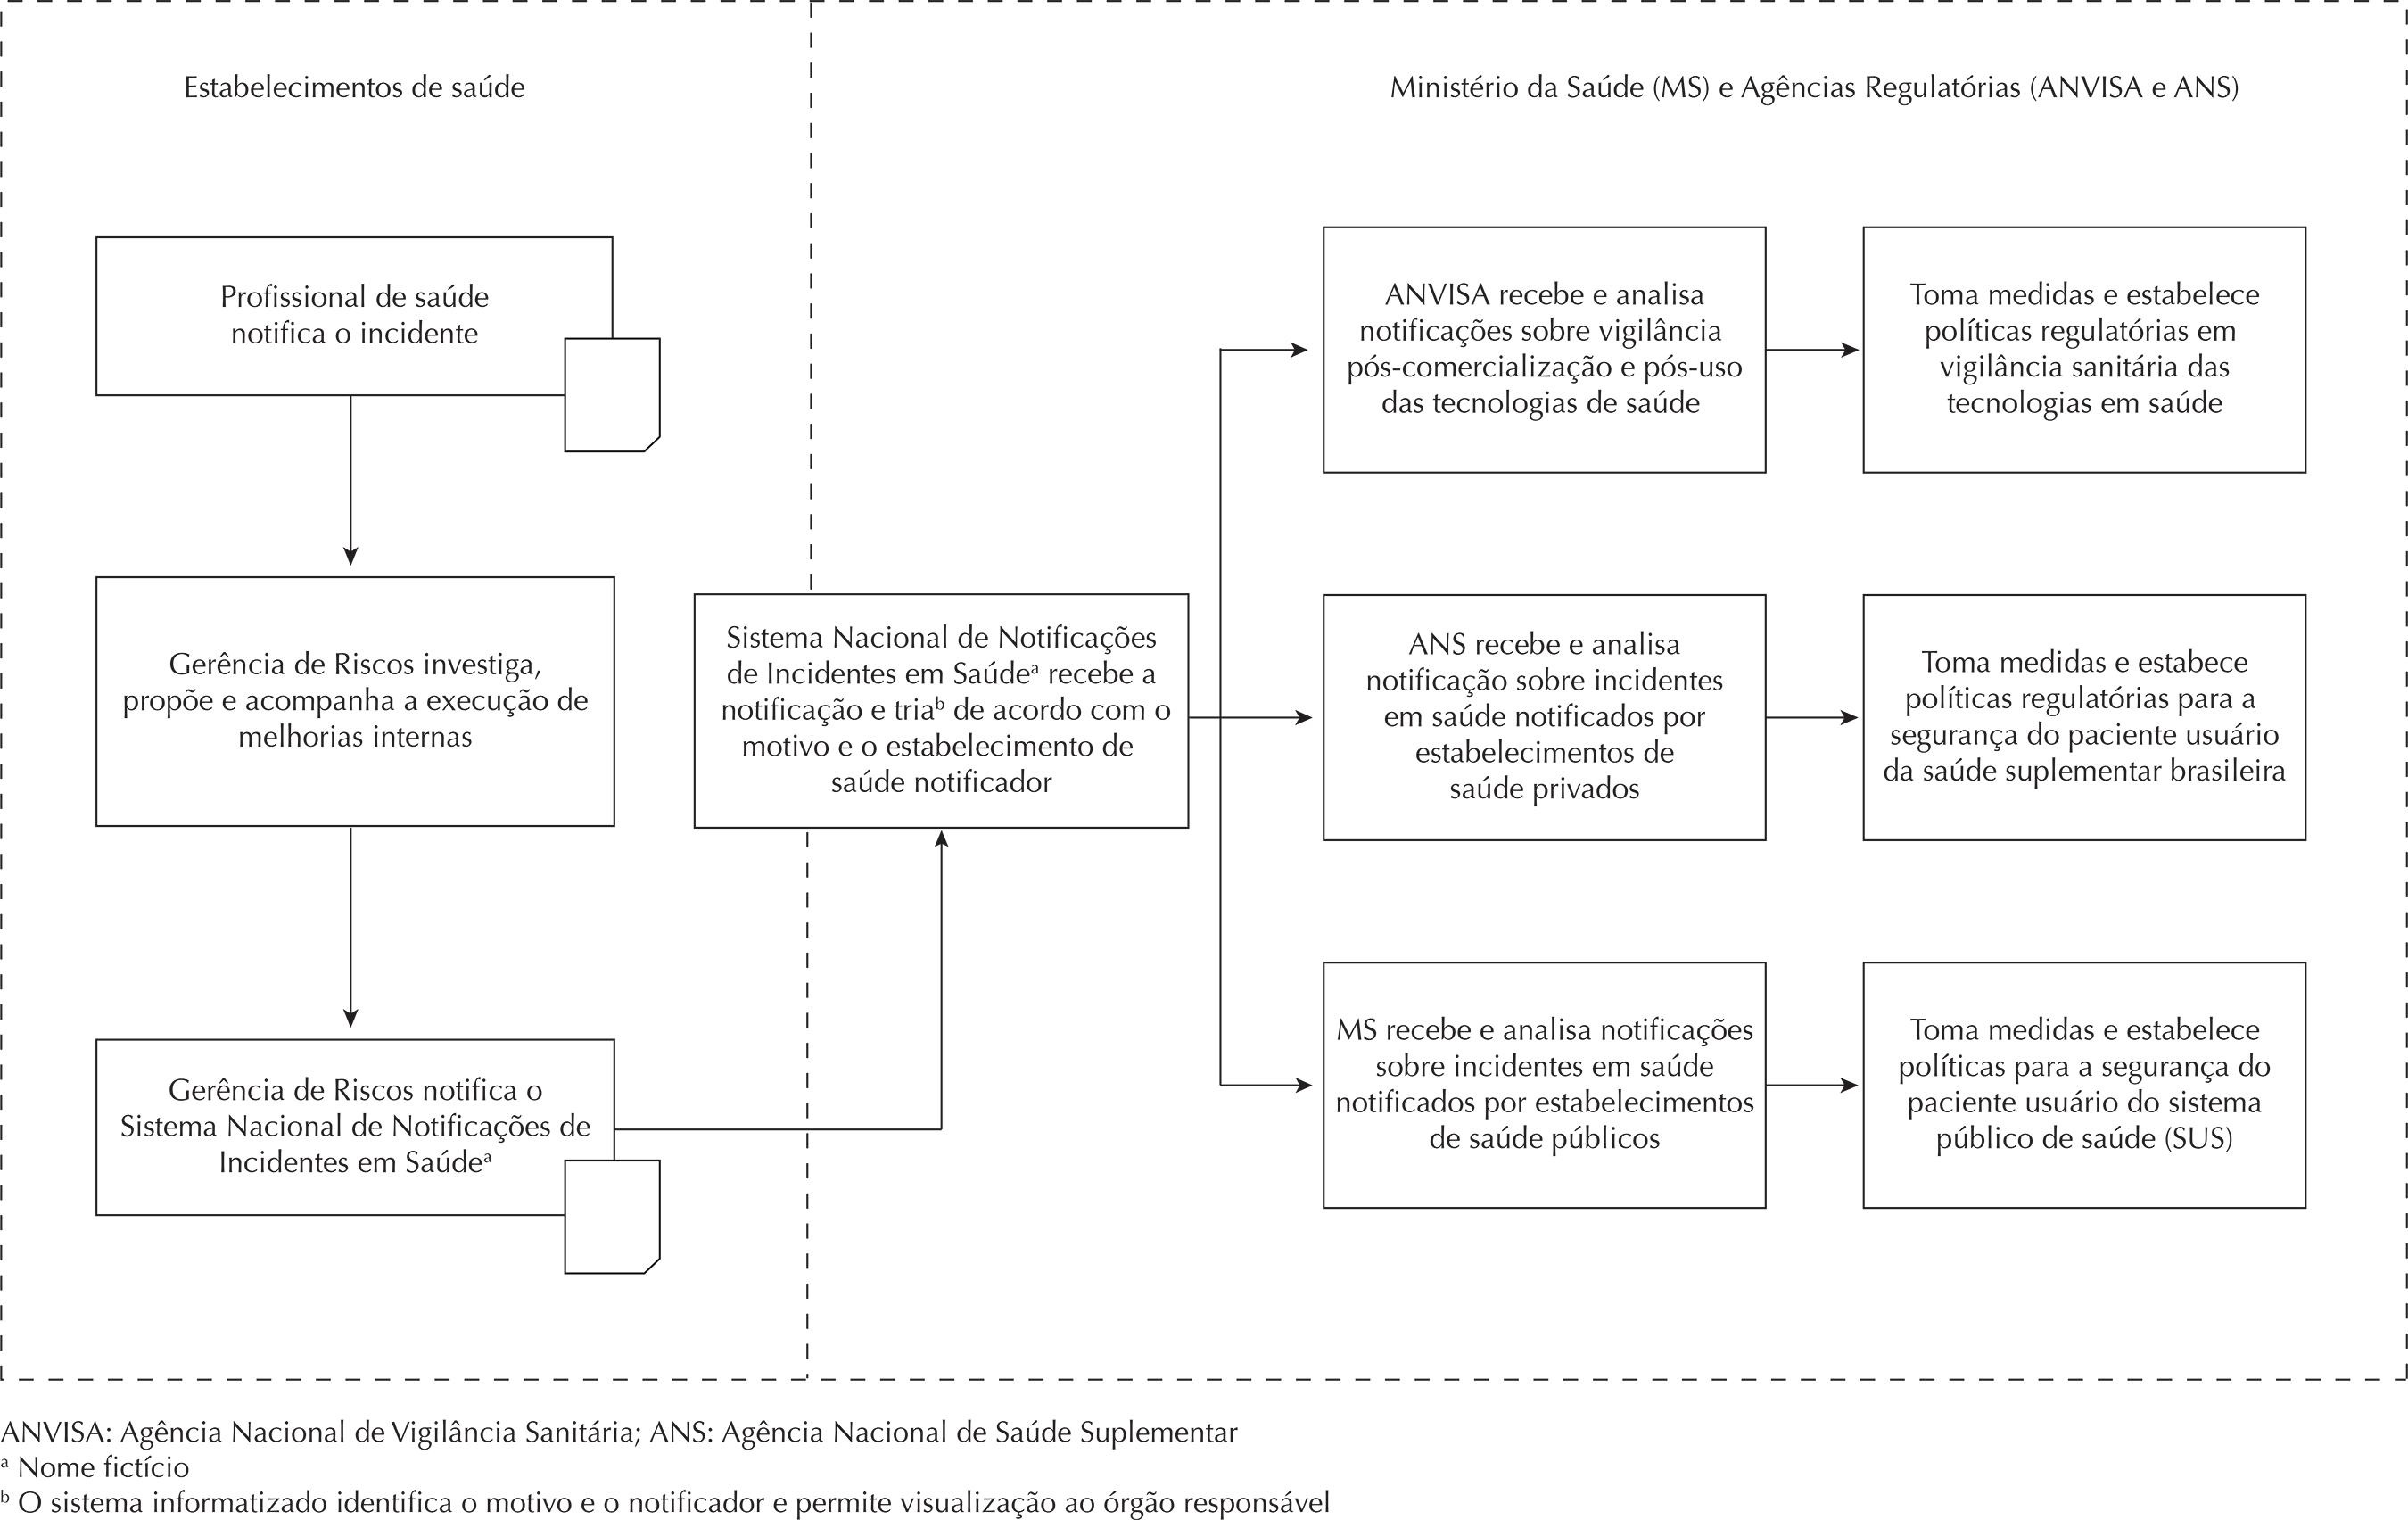
\includegraphics[width=\textwidth]{0034-8910-rsp-47-04-0791-gf01.jpg}
\caption{Fluxo simplificado para o Sistema Nacional de Notificações de
Incidentes em
Saúde.}\label{fig:f01}
\end{figure}

O desenvolvimento e implementação de um sistema informatizado único para receber

\includegraphics[height=.8\baselineskip]{0034-8910-rsp-47-04-0791-g1.jpg}
notificações de todas as instituições de saúde deverá ter como objetivos
facilitar e
agilizar o processo de envio e de tomada de decisões a partir da notificação,
minimizando
riscos e evitando eventos adversos, ampliando a qualidade da assistência e a
segurança dos
pacientes em todos os níveis, da menor clínica de atenção à saúde ao sistema de
saúde
brasileiro; ampliar o conhecimento sobre os riscos e incidentes que ocorrem nas
instituições
brasileiras, direcionando o planejamento de ações dos gestores de saúde;
melhorar a
qualidade dos dados encaminhados; garantir a legibilidade das informações
disponíveis;
preservar a confidencialidade dos notificadores e dados relatados; e, por fim,
reduzir
custos do processo de notificação.

À medida que o sistema seja utilizado com maior frequência e eficácia para o
envio
voluntário de notificações de incidentes, especialmente os potenciais eventos
adversos, a
tomada de decisões quanto às intervenções necessárias para evitar a ocorrência
de danos
poderá ser mais rápida, o que pode reduzir gastos desnecessários com tratamento
de eventos
adversos que poderiam ter sido prevenidos.

Para tanto, a autonomia e pró-atividade das instituições de saúde deve ser
estimulada. Até
que haja a tomada de decisão por parte do governo, as instituições também devem
realizar
ações de melhoria internas, visando à promoção da segurança do paciente e à
qualidade da
atenção. Nesse sentindo, os estabelecimentos de saúde deverão ter acesso ao
sistema
informatizado não somente para o envio de notificações da gerência de riscos
para o sistema
nacional, mas também para que essa gerência se utilize do sistema para receber
as
notificações da equipe de saúde de sua instituição. Adicionalmente, o sistema
deve permitir
que a instituição acompanhe o andamento da análise das informações por ela
encaminhadas ao
sistema nacional.

O sistema informatizado é uma importante estratégia de promoção da qualidade
aliada à
sustentabilidade, pois, ao deixar de utilizar papéis, reduz gastos com materiais
de consumo
e geração de resíduos como os próprios papéis, cartuchos de impressoras e
canetas.
Adicionalmente, há outros aspectos que justificam a implantação de sistemas
informatizados
de notificação, a saber:
\textsuperscript{[}\textsuperscript{5}\textsuperscript{]}

\begin{itemize}
\item
elimina a necessidade de utilização de sistemas de envio de documentos internos
às
instituições e destas para o sistema nacional de notificações, o que reduz o
tempo da
chegada da informação e reduz gastos com o envio delas;

\item
pode-se eliminar a possibilidade de extravio e perda de informações,
especialmente se
estas forem preservadas em bancos de dados redundantes e cópias de segurança,
sem
necessidade de espaço para arquivo físico, além de permitir o manuseio ágil das
informações e a análise de indicadores de gestão;

\item
é possível requerer mais informações sobre os incidentes sem dificultar a coleta
dos
dados, melhorando a qualidade das informações e ampliando a participação dos
profissionais de saúde, o que não é possível com o sistema manuscrito.

\end{itemize}

Quanto aos aspectos sociais da sustentabilidade, reduzir o tempo gasto para o
envio do
relato aumenta a participação dos profissionais de saúde com as notificações,
bem como sua
disponibilidade junto aos pacientes possibilitam o envolvimento do paciente e
seus
cuidadores no processo de monitorização de riscos e incidentes em saúde. Em uma
política
nacional, esses atores são fontes importantes de notificação voluntária. Com o
sistema
informatizado de notificações em plataforma web, é possível que qualquer pessoa
com acesso à
internet faça uma notificação.

Países que já possuem política nacional de segurança do paciente, como
Inglaterra, Estados
Unidos, Austrália e Canadá, já permitem que os usuários do sistema e seus
cuidadores façam
notificações sobre riscos e incidentes que vivenciaram ou perceberam em serviços
de saúde,
sendo fundamentais para promoção da qualidade da assistência.

O sistema nacional de notificações deveria, ainda, estar hospedado em um site
interativo
que disponibilizasse gratuitamente notícias, dicas de segurança, informações
sobre eventos
adversos, protocolos sobre como implementar um programa de segurança nos
serviços de saúde,
cursos e palestras \textit{online}
, como o \textit{Institute for Health
Improvement}
tem feito nos Estados Unidos para os hospitais americanos. Esse
portal teria como dupla função manter e estimular a adesão das instituições, e
difundir e
estimular a adoção de práticas seguras por meio do intercâmbio entre elas.

A implantação do sistema informatizado de notificações sobre incidentes na saúde
como base
para a cultura de segurança do paciente no sistema de saúde brasileiro parece
ser uma
estratégia viável e necessária para a qualificação da assistência, com a qual os
gestores
conhecerão os incidentes que ocorrem na prestação de assistência aos usuários do
sistema, em
instituições públicas e privadas, de forma sistematizada, sem depender de que
pesquisas
sejam realizadas exclusivamente para esse fim. Desse modo, nortear-se-á o
delineamento de
estratégias de gestão de riscos para a segurança do paciente, ampliando a
qualidade dos
serviços ofertados à população brasileira.

\section{DESTAQUES}
Recentemente, foi lançado pelo Ministério da Saúde o Programa Nacional de
Segurança do
Paciente para que ações de segurança do paciente fossem promovidas no âmbito do
Sistema
Único de Saúde. É louvável essa iniciativa e foi o maior foco de discussão do
artigo, o qual
aborda importantes pontos que não foram incluídos no citado Programa. Esses
pontos
referem-se à forma com que o Governo pretende remunerar as instituições que
obtiverem os
melhores resultados na prestação de serviços e também como serão tratadas as
informações
advindas de notifi cações, de forma que o conhecimento gerado promova a melhoria
efetiva dos
serviços prestados pelo Sistema Único de Saúde.

O artigo faz refl exão à luz da melhoria da política de saúde para a segurança
do paciente,
onde foi possível verificar que ações para a cultura de segurança podem
proliferar e gerar
bons resultados também em hospitais públicos. Assim, traz à luz discussões
importantes para
todas as instituições e especialmente para gestores do sistema de forma a
aprimorar o
Programa Nacional e desencadear a melhoria contínua dos serviços centrada no
paciente.

Profa. Rita de Cássia Barradas Barata

Editora Científica

\section*{REFERÊNCIAS}
\begin{itemize}

\item[1] . Almeida-Filho N. Ensino superior e os serviços de saúde no Brasil.
\textit{Lancet}
. 2011;6-7.

\item[2] . Bentzen N. WONCA dictionary of general/family practice. Copenhagen:
Maanedskift Lager; 2003.

\item[3] . Berlowitz D, Burgess Jr JF, Young GJ. Improving quality of care:
emerging
evidence on pay-for-performance. \textit{Med Care Res Rev}
. 2006;63(1
Suppl):73S-95S.

\item[4] . Capucho HC. Near miss: quase erro ou potencial evento adverso?
\textit{Rev
Latino-Am Enferm}
. 2011;19(5):1272-3.
DOI:10.1590/S0104-11692011000500027

\item[5] . Capucho HC, Arnas ER, Cassiani SHBD. Segurança do paciente:
comparação
entre notificações voluntárias manuscritas e informatizadas sobre incidentes em
saúde.
\textit{Rev Gaucha Enferm}
. 2013;34(1):164-72.
DOI:10.1590/S1983-14472013000100021

\item[6] . Constance HF, Yee Wei L, Mattke S, Damberg C, Shekelle PG. Systematic
Review: The Evidence That Publishing Patient Care Performance Data Improves
Quality of
Care. \textit{Ann Intern Med}
. 2008;15(148):111-123.

\item[7] . Escrivao Jr A, Koyama MF. O relacionamento entre hospitais e
operadoras de
planos de saúde no âmbito do Programa de Qualificação da Saúde Suplementar da
ANS.
\textit{Cienc Saude Coletiva}
. 2007;12(4):903-14.
DOI:10.1590/S1413-81232007000400012

\item[8] . Fisher ES. Paying for Performance - Risks and Recommendations.
\textit{New
Eng J Med}
. 2006;355(18):1845-7. DOI:10.1056/NEJMp068221

\item[9] . Fung CH, Lim YW, Mattke S, Damberg C, Shekelle PG. Systematic Review:
The
Evidence That Publishing Patient Care Performance Data Improves Quality of Care.
\textit{Ann Intern Med}
. 2008;148(2):111-23.
DOI:10.7326/0003-4819-148-2-200801150-00006

\item[10] . Gouvêa CSDD, Travassos C. Indicadores de segurança do paciente para
hospitais de pacientes agudos: revisão sistemática. \textit{Cad Saude Publica}
.
2010;26(6):1061-78. DOI:10.1590/S0102-311X2010000600002

\item[11] . Kohn LT, Corrigan JM, Donaldson MS. To err is human: building a
safer
health system. 2.ed. Washington: National Academy of Sciences; 1999.

\item[12] . McDonald R, Roland M. Pay for performance in primary care in England
and
California: comparison of unintended consequences. \textit{Ann Fam Med}
.
2009;7(2):121-7. DOI:10.1370/afm.946

\item[13] . Mendes W, Martins M, Rozenfeld S, Travassos C. The assessment of
adverse
events in hospitals in Brazil. \textit{Int J Qual Health Care}
.
2009;21(4):279-84. DOI:10.1093/intqhc/mzp022

\item[14] . Miasso, AI, Grou CR, Cassiani SHB, Silva AEBC, Fakih FT. Erros de
medicação: tipos, fatores causais e providencias em quatro hospitais
brasileiros.
\textit{Rev Esc Enferm USP}
. 2006:40(4):524-32.
DOI:10.1590/S0080-62342006000400011

\item[15] . Novaes HM. O processo de acreditação dos serviços de saúde.
\textit{Rev
Adm Saude}
. 2007;9(37):133-40.

\item[16] . Paim J, Travassos C, Almeida C, Bahia L, Macinko J. O sistema de
saúde
brasileiro: história, avanços e desafios. \textit{Lancet}
.
2011;11-31.

\item[17] . Shoyer AL, London MJ, VillaNueva CB, Sethi GK, Marshall G, Moritz
TE, et
al. The processes, structures, and outcomes of care in cardiac surgery study an
overview.
\textit{Med Care}
. 1995;33(10):OS1-4.
DOI:10.1097/00005650-199510001-00001

\item[18] . Thomas AN, Panchagnula U. Medication-related patient safety
incidents in
critical care: a review of reports to the UK National Patient Safety Agency.
\textit{Anaesthesia}
. 2008;63(7):726-33.
DOI:10.1111/j.1365-2044.2008.05485.x

\item[19] . Unruh LY, Zhang NJ. Nurse Staffing and patient safety in hospitals:
new
variable and longitudinal approaches. \textit{Nurs Res}
. 2012;61(1):3-12.
DOI:10.1097/NNR.0b013e3182358968

\item[20] . Victora CG, Barreto ML, Leal MC, Monteiro CA, Schmidt MI, Paim J, et
al.
Condições de saúde e inovações nas políticas de saúde no Brasil: o caminho a
percorrer.
\textit{Lancet}
. 2011;90-102.

\item[21] . Vincent C. Segurança do paciente. Orientações para evitar eventos
adversos. São Caetano do Sul: Editora Yendis; 2009.

\item[22] . Vincent C, Woloshynowych M. Adverse events in British hospitals:
preliminary retrospective record review. \textit{BMJ}
. 2001;322(7285):517-9.
DOI:10.1136/bmj.322.7285.517

\item[23] . World Health Organization. The conceptual framework for the
international
classification for patient safety. Version 1.1. Final technical report. Chapter
3. The
international classification for patient safety. Key concepts and preferred
terms. Geneva;
2009 [citado 2011 jul 04]. Disponível em:
http://www.who.int/patientsafety/taxonomy/icps\_{}chapter3.pdf

\end{itemize}

   \section*{Metadados não aplicados}
    \begin{itemize}
    \ifdef{\lingua}{\item[\textbf{língua do artigo}] \lingua}{}
    \ifdef{\journalid}{\item[\textbf{journalid}] \journalid}{}
    \ifdef{\journaltitle}{\item[\textbf{journaltitle}] \journaltitle}{}
    \ifdef{\journalsubtitle}{\item[\textbf{journalsubtitle}] \journalsubtitle}{}
    \ifdef{\historydateaccepted}{\item[\textbf{historydateaccepted}] \historydateaccepted}{}
    \ifdef{\historydatereceived}{\item[\textbf{historydatereceived}] \historydatereceived}{}
    \ifdef{\ack}{\item[\textbf{ack}] \ack}{}
    \ifdef{\transjournaltitle}{\item[\textbf{journaltitle}] \journaltitle}{}
    \ifdef{\transjournalsubtitle}{\item[\textbf{journalsubtitle}] \journaltitle}{}
    \ifdef{\abbrevjournaltitle}{\item[\textbf{abbrevjournaltitle}] \abbrevjournaltitle}{}
    \ifdef{\issnppub}{\item[\textbf{issnppub}] \issnppub}{}
    \ifdef{\issnepub}{\item[\textbf{issnepub}] \issnepub}{}
    \ifdef{\alttitleauthor}{\item[\textbf{alttitle}] \alttitleauthor}{}
    \ifdef{\alttitle}{\item[\textbf{alttitleauthor}] \alttitle}{}
    \ifdef{\publishername}{\item[\textbf{publishername}] \publishername}{}
    \ifdef{\publisherid}{\item[\textbf{publisherid}] \publisherid}{}
    \ifdef{\subject}{\item[\textbf{subject}] \subject}{} 
    \ifdef{\transtitle}{\item[\textbf{transtitle}] \transtitle}{}
    \ifdef{\authornotes}{\item[\textbf{authornotes}] \authornotes}{}
    \ifdef{\articleid}{\item[\textbf{articleid}] \articleid}{}
    \ifdef{\articledoi}{\item[\textbf{articledoi}] \articledoi}{}
    \ifdef{\volume}{\item[\textbf{volume}] \volume}{}
    \ifdef{\issue}{\item[\textbf{issue}] \issue}{}
    \ifdef{\fpage}{\item[\textbf{fpage}] \fpage}{}
    \ifdef{\lpage}{\item[\textbf{lpage}] \lpage}{}
    \ifdef{\permissions}{\item[\textbf{permissions}] \permissions}{}
    \ifdef{\copyrightyear}{\item[\textbf{copyrightyear}] \copyrightyear}{}

    \end{itemize}
\end{document}
